\documentclass[]{article}
\usepackage{lmodern}
\usepackage{amssymb,amsmath}
\usepackage{ifxetex,ifluatex}
\usepackage{fixltx2e} % provides \textsubscript
\ifnum 0\ifxetex 1\fi\ifluatex 1\fi=0 % if pdftex
  \usepackage[T1]{fontenc}
  \usepackage[utf8]{inputenc}
\else % if luatex or xelatex
  \ifxetex
    \usepackage{mathspec}
  \else
    \usepackage{fontspec}
  \fi
  \defaultfontfeatures{Ligatures=TeX,Scale=MatchLowercase}
\fi
% use upquote if available, for straight quotes in verbatim environments
\IfFileExists{upquote.sty}{\usepackage{upquote}}{}
% use microtype if available
\IfFileExists{microtype.sty}{%
\usepackage{microtype}
\UseMicrotypeSet[protrusion]{basicmath} % disable protrusion for tt fonts
}{}
\usepackage[margin=1in]{geometry}
\usepackage{hyperref}
\hypersetup{unicode=true,
            pdftitle={Processing, cleaning and saving NZ GREEN Grid project time use diary data},
            pdfauthor={Ben Anderson (b.anderson@soton.ac.uk, @dataknut)},
            pdfborder={0 0 0},
            breaklinks=true}
\urlstyle{same}  % don't use monospace font for urls
\usepackage{longtable,booktabs}
\usepackage{graphicx,grffile}
\makeatletter
\def\maxwidth{\ifdim\Gin@nat@width>\linewidth\linewidth\else\Gin@nat@width\fi}
\def\maxheight{\ifdim\Gin@nat@height>\textheight\textheight\else\Gin@nat@height\fi}
\makeatother
% Scale images if necessary, so that they will not overflow the page
% margins by default, and it is still possible to overwrite the defaults
% using explicit options in \includegraphics[width, height, ...]{}
\setkeys{Gin}{width=\maxwidth,height=\maxheight,keepaspectratio}
\IfFileExists{parskip.sty}{%
\usepackage{parskip}
}{% else
\setlength{\parindent}{0pt}
\setlength{\parskip}{6pt plus 2pt minus 1pt}
}
\setlength{\emergencystretch}{3em}  % prevent overfull lines
\providecommand{\tightlist}{%
  \setlength{\itemsep}{0pt}\setlength{\parskip}{0pt}}
\setcounter{secnumdepth}{5}
% Redefines (sub)paragraphs to behave more like sections
\ifx\paragraph\undefined\else
\let\oldparagraph\paragraph
\renewcommand{\paragraph}[1]{\oldparagraph{#1}\mbox{}}
\fi
\ifx\subparagraph\undefined\else
\let\oldsubparagraph\subparagraph
\renewcommand{\subparagraph}[1]{\oldsubparagraph{#1}\mbox{}}
\fi

%%% Use protect on footnotes to avoid problems with footnotes in titles
\let\rmarkdownfootnote\footnote%
\def\footnote{\protect\rmarkdownfootnote}

%%% Change title format to be more compact
\usepackage{titling}

% Create subtitle command for use in maketitle
\newcommand{\subtitle}[1]{
  \posttitle{
    \begin{center}\large#1\end{center}
    }
}

\setlength{\droptitle}{-2em}
  \title{Processing, cleaning and saving NZ GREEN Grid project time use diary
data}
  \pretitle{\vspace{\droptitle}\centering\huge}
  \posttitle{\par}
  \author{Ben Anderson
(\href{mailto:b.anderson@soton.ac.uk}{\nolinkurl{b.anderson@soton.ac.uk}},
\texttt{@dataknut})}
  \preauthor{\centering\large\emph}
  \postauthor{\par}
  \predate{\centering\large\emph}
  \postdate{\par}
<<<<<<< HEAD
  \date{Last run at: 2018-05-22 10:14:51}
=======
  \date{Last run at: 2018-05-22 10:08:59}
>>>>>>> 8aad2b775c17c569a76cca0fc63e94e74b84bba0


\begin{document}
\maketitle

{
\setcounter{tocdepth}{2}
\tableofcontents
}
\newpage

\section{Citation}\label{citation}

If you wish to use any of the material from this report please cite as:

\begin{itemize}
\tightlist
\item
  Anderson, B. (2018) Processing, cleaning and saving NZ GREEN Grid
  project time use diary data, University of Otago: Dunedin, NZ.
\end{itemize}

\newpage

\section{Introduction}\label{introduction}

Report circulation:

\begin{itemize}
\tightlist
\item
  Restricted to:
  \href{https://www.otago.ac.nz/centre-sustainability/research/energy/otago050285.html}{NZ
  GREEn Grid} project partners and contractors.
\end{itemize}

\subsection{Purpose}\label{purpose}

This report is intended to:

\begin{itemize}
\tightlist
\item
  load and clean the two time use survey datasets
\item
  save the cleaned data out to /Volumes/hum-csafe/Research
  Projects/GREEN Grid/Clean\_data/safe/TUD/ as two seperate files, one
  for each survey
\item
  produce summary data quality statistics
\end{itemize}

\subsection{Requirements:}\label{requirements}

Time use survey data held in /Volumes/hum-csafe/Research Projects/GREEN
Grid/\_RAW DATA/Time Use Diaries/:

\begin{itemize}
\tightlist
\item
  PowerCo
\item
  Unison
\end{itemize}

A lookup table to correct mis-coding of household IDs
(/Volumes/hum-csafe/Research Projects/GREEN Grid/\_RAW
DATA/TUD\_2\_GridSpyLookup.xlsx).

\subsection{History}\label{history}

Generally tracked via our git.soton
\href{https://git.soton.ac.uk/ba1e12/nzGREENGrid}{repo}:

\begin{itemize}
\tightlist
\item
  \href{https://git.soton.ac.uk/ba1e12/nzGREENGrid/commits/master}{history}
\item
  \href{https://git.soton.ac.uk/ba1e12/nzGREENGrid/issues}{issues}
\end{itemize}

\subsection{Support}\label{support}

This work was supported by:

\begin{itemize}
\tightlist
\item
  The \href{https://www.otago.ac.nz/}{University of Otago}
\item
  The New Zealand \href{http://www.mbie.govt.nz/}{Ministry of Business,
  Innovation and Employment (MBIE)}
\item
  \href{http://www.energy.soton.ac.uk/tag/spatialec/}{SPATIALEC} - a
  \href{http://ec.europa.eu/research/mariecurieactions/about-msca/actions/if/index_en.htm}{Marie
  Skłodowska-Curie Global Fellowship} based at the University of Otago's
  \href{http://www.otago.ac.nz/centre-sustainability/staff/otago673896.html}{Centre
  for Sustainability} (2017-2019) \& the University of Southampton's
  Sustainable Energy Research Group (2019-202).
\end{itemize}

This work is (c) 2018 the University of Southampton.

We do not `support' the code but if you have a problem check the
\href{https://git.soton.ac.uk/ba1e12/nzGREENGrid/issues}{issues} on our
\href{https://git.soton.ac.uk/ba1e12/nzGREENGrid}{repo} and if it
doesn't already exist, open one. We might be able to fix it :-)

\section{PowerCo}\label{powerco}

This consists of 1 file found in /Volumes/hum-csafe/Research
Projects/GREEN Grid/\_RAW DATA/Time Use Diaries/Powerco/Powerco
Annexes/:

\begin{itemize}
\tightlist
\item
  TUD (Merged data)\_BA.csv
\end{itemize}

This is a version of TUD (Merged data).csv with:

\begin{itemize}
\tightlist
\item
  small edits to correct dates
\item
  redundant rows removed from file header
\end{itemize}

\subsection{Load \& process}\label{load-process}

\begin{verbatim}
## [1] "Found 352 rows of data"
\end{verbatim}

\begin{verbatim}
## [1] "Removing unsafe vars: RowNum"      
## [2] "Removing unsafe vars: Name"        
## [3] "Removing unsafe vars: EmailAddress"
\end{verbatim}

\begin{verbatim}
## [1] "Fixing variable names"
\end{verbatim}

\begin{verbatim}
## [1] "Fixing dates"
\end{verbatim}

\begin{verbatim}
## [1] "Fixing hhID"
\end{verbatim}

The following table summarises the PowerCo cleaned diary data. In theory
we should have 1 diary per day per person - so a 1 person household
should have produced 7 diaries\ldots{} A 3 person household would
produce 14 if there were two adults and 1 child (for example).

\begin{quote}
What was the age cut off for diary completion?
\end{quote}

\begin{longtable}[]{@{}lrrll@{}}
\caption{Summary of PowerCo diaries by household}\tabularnewline
\toprule
hhID & nDiaries & familySize & minDiaryDate &
maxDiaryDate\tabularnewline
\midrule
\endfirsthead
\toprule
hhID & nDiaries & familySize & minDiaryDate &
maxDiaryDate\tabularnewline
\midrule
\endhead
rf\_06 & 14 & 2.000000 & 2014-08-23 & 2014-08-29\tabularnewline
rf\_07 & 14 & 3.000000 & 2014-08-25 & 2014-08-31\tabularnewline
rf\_08 & 7 & 1.000000 & 2014-08-23 & 2014-08-29\tabularnewline
rf\_09 & 14 & 2.000000 & 2014-08-23 & 2014-08-29\tabularnewline
rf\_10 & 14 & 2.000000 & 2014-08-23 & 2014-08-29\tabularnewline
rf\_11 & 7 & 1.000000 & 2014-08-23 & 2014-08-29\tabularnewline
rf\_12 & 14 & 3.000000 & 2014-08-23 & 2014-08-29\tabularnewline
rf\_13 & 12 & 2.000000 & 2014-08-23 & 2014-08-29\tabularnewline
rf\_14 & 43 & 5.906977 & 2014-08-23 & 2014-08-29\tabularnewline
rf\_15 & 14 & 3.000000 & 2014-08-23 & 2014-08-29\tabularnewline
rf\_16 & 14 & 3.000000 & 2014-08-23 & 2014-08-29\tabularnewline
rf\_17 & 14 & 2.000000 & 2014-08-26 & 2014-09-01\tabularnewline
rf\_18 & 14 & 2.000000 & 2014-08-23 & 2014-08-29\tabularnewline
rf\_19 & 14 & 3.000000 & 2014-08-23 & 2014-08-29\tabularnewline
rf\_20 & 35 & 6.000000 & 2014-08-23 & 2014-08-29\tabularnewline
rf\_21 & 14 & 2.000000 & 2014-08-23 & 2014-08-29\tabularnewline
rf\_22 & 14 & 2.000000 & 2014-08-23 & 2014-08-29\tabularnewline
rf\_23 & 14 & 4.000000 & 2014-08-23 & 2014-08-29\tabularnewline
rf\_24 & 28 & 4.000000 & 2014-08-23 & 2014-08-29\tabularnewline
rf\_25 & 21 & 4.000000 & 2014-08-23 & 2014-08-29\tabularnewline
rf\_26 & 7 & 1.000000 & 2014-08-23 & 2014-08-29\tabularnewline
rf\_27 & 10 & 4.000000 & 2014-08-23 & 2014-08-29\tabularnewline
\bottomrule
\end{longtable}

\begin{verbatim}
## [1] "Saving PowerCo cleaned time use diary to /Volumes/hum-csafe/Research Projects/GREEN Grid/Clean_data/safe/TUD/powerCoTUDsafe.csv"
\end{verbatim}

\begin{verbatim}
## [1] "Done"
\end{verbatim}

\subsection{Tests}\label{tests}

Should all be in August 2014\ldots{}

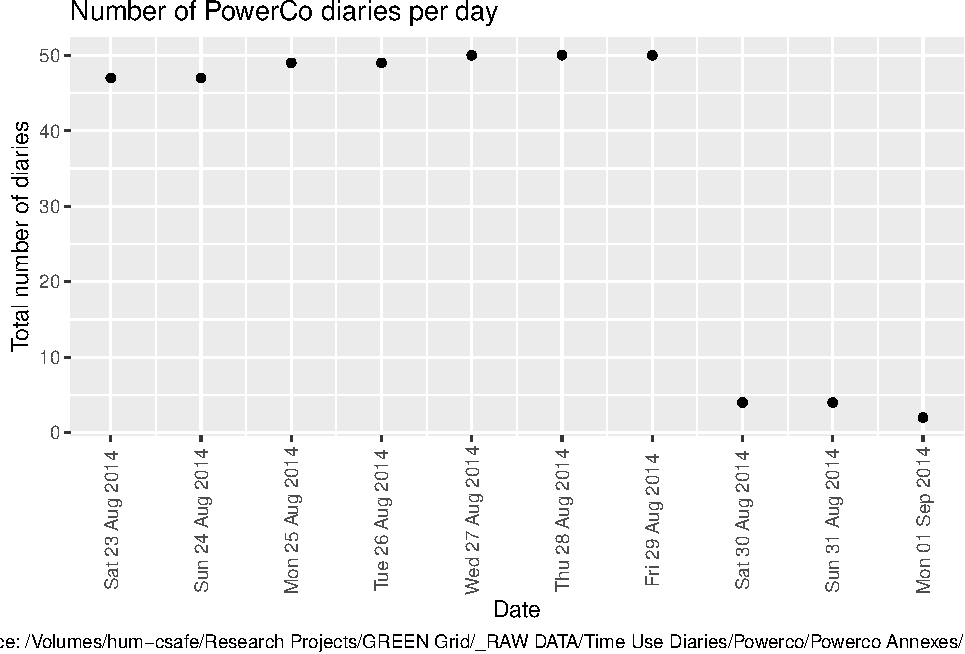
\includegraphics{processNZGGTUDData_files/figure-latex/powerCoDiaryPlot-1.pdf}

\begin{verbatim}
## Saving 6.5 x 4.5 in image
\end{verbatim}

In total we have 352 diaries from 22 PowerCo households.

\section{Unison}\label{unison}

This consists of 5 files found in /Volumes/hum-csafe/Research
Projects/GREEN Grid/\_RAW DATA/Time Use Diaries/Unison/Unison Raw
Data/Raw data with paper diaries included/Cleaned excel data files/:

\begin{itemize}
\tightlist
\item
  TUDAdult\_ONE\_Child\_Unison\_forSAS\_BA.xlsx
\item
  TUDAdult\_TWO\_Children\_Unison\_forSAS\_BA.xlsx
\item
  TUDAdult-THREE-Children-Unison\_forSAS\_BA.xlsx
\item
  TUDAdult-Unison-forSAS\_BA.xlsx
\item
  TUDTeenagerorChild-Unison\_forSAS\_BA.xlsx
\end{itemize}

As before these are copies of the original versions with slight editing
to correct dates and for ease of processing. The relationship between
them is currently unclear!

\subsection{Load \& process}\label{load-process-1}

\begin{verbatim}
## [1] "Found 352 rows in total"
\end{verbatim}

\begin{verbatim}
## [1] "Removing unsafe vars: Name"        
## [2] "Removing unsafe vars: EmailAddress"
## [3] "Removing unsafe vars: IPAddress"
\end{verbatim}

\begin{verbatim}
## [1] "Fixing variable names"
\end{verbatim}

\begin{verbatim}
## [1] "Fixing hhID"
\end{verbatim}

The following table lists rows where the diary date did not parse (for
error checking).

<<<<<<< HEAD
\begin{longtable}[]{@{}llllll@{}}
=======
\begin{longtable}[]{@{}lllll@{}}
>>>>>>> 8aad2b775c17c569a76cca0fc63e94e74b84bba0
\caption{Test diaryDates that did not parse}\tabularnewline
\toprule
ResponseID & r\_diaryDate & code & tudCode & StartDate &
EndDate\tabularnewline
\midrule
\endfirsthead
\toprule
ResponseID & r\_diaryDate & code & tudCode & StartDate &
EndDate\tabularnewline
\midrule
\endhead
NA & NA & NA & NA & NA & NA\tabularnewline
NA & NA & NA & NA & NA & NA\tabularnewline
NA & NA & NA & NA & 2015-07-21 21:12:46 & 2015-07-21
21:13:00\tabularnewline
\bottomrule
\end{longtable}

The following table reports any diaries where the dates were manually
edited before loading.

\begin{longtable}[]{@{}llll@{}}
\caption{Report diaries with edited diary dates (done in .xlsx before
loading)}\tabularnewline
\toprule
r\_diaryDate & tudCode & dateNote & sourceFile\tabularnewline
\midrule
\endfirsthead
\toprule
r\_diaryDate & tudCode & dateNote & sourceFile\tabularnewline
\midrule
\endhead
2015-07-20 & 28 & imputed &
TUDAdult\_ONE\_Child\_Unison\_forSAS\_BA.xlsx\tabularnewline
2015-07-21 & 28 & imputed &
TUDAdult\_ONE\_Child\_Unison\_forSAS\_BA.xlsx\tabularnewline
2015-07-20 & 33 & imputed &
TUDAdult\_ONE\_Child\_Unison\_forSAS\_BA.xlsx\tabularnewline
2015-07-20 & 39 & imputed &
TUDAdult\_ONE\_Child\_Unison\_forSAS\_BA.xlsx\tabularnewline
2015-07-23 & 39 & imputed &
TUDAdult\_ONE\_Child\_Unison\_forSAS\_BA.xlsx\tabularnewline
2015-07-24 & 39 & imputed &
TUDAdult\_ONE\_Child\_Unison\_forSAS\_BA.xlsx\tabularnewline
2015-07-26 & 39 & imputed &
TUDAdult\_ONE\_Child\_Unison\_forSAS\_BA.xlsx\tabularnewline
2015-07-20 & 39 & imputed &
TUDAdult\_ONE\_Child\_Unison\_forSAS\_BA.xlsx\tabularnewline
2015-07-20 & 41 & might actually be the 20th &
TUDAdult\_TWO\_Children\_Unison\_forSAS\_BA.xlsx\tabularnewline
2015-07-21 & 41 & might actually be the 21st &
TUDAdult\_TWO\_Children\_Unison\_forSAS\_BA.xlsx\tabularnewline
2015-07-20 & 41 & imputed from StartDate &
TUDAdult\_TWO\_Children\_Unison\_forSAS\_BA.xlsx\tabularnewline
2015-07-21 & 41 & imputed from StartDate &
TUDAdult\_TWO\_Children\_Unison\_forSAS\_BA.xlsx\tabularnewline
2015-07-22 & 41 & imputed from StartDate &
TUDAdult\_TWO\_Children\_Unison\_forSAS\_BA.xlsx\tabularnewline
2015-07-23 & 41 & imputed from StartDate &
TUDAdult\_TWO\_Children\_Unison\_forSAS\_BA.xlsx\tabularnewline
2015-07-24 & 41 & imputed from StartDate &
TUDAdult\_TWO\_Children\_Unison\_forSAS\_BA.xlsx\tabularnewline
2015-07-25 & 41 & imputed from StartDate &
TUDAdult\_TWO\_Children\_Unison\_forSAS\_BA.xlsx\tabularnewline
2015-07-26 & 41 & imputed from StartDate &
TUDAdult\_TWO\_Children\_Unison\_forSAS\_BA.xlsx\tabularnewline
2015-07-21 & 31 & corrected to July from Feb &
TUDTeenagerorChild-Unison\_forSAS\_BA.xlsx\tabularnewline
2015-07-26 & 45 & 25/7/2015 missing in original &
TUDTeenagerorChild-Unison\_forSAS\_BA.xlsx\tabularnewline
\bottomrule
\end{longtable}

The following table summarises the Unison diary data.

\begin{longtable}[]{@{}lrll@{}}
\caption{Summary of Unison diaries by household}\tabularnewline
\toprule
tudCode & nDiaries & minDiaryDate & maxDiaryDate\tabularnewline
\midrule
\endfirsthead
\toprule
tudCode & nDiaries & minDiaryDate & maxDiaryDate\tabularnewline
\midrule
\endhead
NA & 3 & NA & NA\tabularnewline
28 & 21 & 2015-07-20 & 2015-07-26\tabularnewline
29 & 14 & 2015-07-20 & 2015-07-26\tabularnewline
30 & 14 & 2015-07-20 & 2015-07-26\tabularnewline
31 & 21 & 2015-07-20 & 2015-07-26\tabularnewline
32 & 21 & 2015-07-20 & 2015-07-26\tabularnewline
33 & 14 & 2015-07-20 & 2015-07-26\tabularnewline
34 & 14 & 2015-07-20 & 2015-07-26\tabularnewline
35 & 14 & 2015-07-20 & 2015-07-26\tabularnewline
36 & 14 & 2015-07-20 & 2015-07-26\tabularnewline
37 & 14 & 2015-07-20 & 2015-07-26\tabularnewline
38 & 21 & 2015-07-20 & 2015-07-26\tabularnewline
39 & 21 & 2015-07-20 & 2015-07-26\tabularnewline
40 & 14 & 2015-07-20 & 2015-07-26\tabularnewline
41 & 21 & 2015-07-20 & 2015-07-26\tabularnewline
42 & 21 & 2015-07-20 & 2015-07-26\tabularnewline
43 & 14 & 2015-08-03 & 2015-08-09\tabularnewline
44 & 14 & 2015-07-20 & 2015-07-26\tabularnewline
45 & 37 & 2015-07-20 & 2015-07-26\tabularnewline
46 & 11 & 2015-07-20 & 2015-07-26\tabularnewline
47 & 14 & 2015-07-20 & 2015-07-26\tabularnewline
\bottomrule
\end{longtable}

Note thaty the tudCodes found in the .csv files are \emph{not} the
gridSpy household ids, we need to create these from the unison sheet in
/Volumes/hum-csafe/Research Projects/GREEN Grid/\_RAW
DATA/TUD\_2\_GridSpyLookup.xlsx.

\begin{longtable}[]{@{}rll@{}}
\caption{Unison linking table}\tabularnewline
\toprule
CODE & tag\_gridSpy\_Hhid & source\tabularnewline
\midrule
\endfirsthead
\toprule
CODE & tag\_gridSpy\_Hhid & source\tabularnewline
\midrule
\endhead
28 & rf\_33 & unison\tabularnewline
29 & rf\_46 & unison\tabularnewline
30 & rf\_37 & unison\tabularnewline
31 & rf\_28 & unison\tabularnewline
32 & rf\_39 & unison\tabularnewline
33 & rf\_29 & unison\tabularnewline
34 & rf\_30 & unison\tabularnewline
35 & rf\_31 & unison\tabularnewline
36 & rf\_43 & unison\tabularnewline
37 & rf\_35 & unison\tabularnewline
38 & rf\_44 & unison\tabularnewline
39 & rf\_41 & unison\tabularnewline
40 & rf\_36 & unison\tabularnewline
41 & rf\_42 & unison\tabularnewline
42 & rf\_34 & unison\tabularnewline
43 & rf\_38 & unison\tabularnewline
43 & rf\_38 & unison\tabularnewline
44 & rf\_32 & unison\tabularnewline
45 & rf\_47 & unison\tabularnewline
46 & rf\_45 & unison\tabularnewline
47 & rf\_40 & unison\tabularnewline
\bottomrule
\end{longtable}

\begin{longtable}[]{@{}llr@{}}
\caption{Check linkage: there should be n * 7 diaries for each
combination}\tabularnewline
\toprule
linkCode & hhID & nDiaries\tabularnewline
\midrule
\endfirsthead
\toprule
linkCode & hhID & nDiaries\tabularnewline
\midrule
\endhead
28 & rf\_33 & 21\tabularnewline
29 & rf\_46 & 14\tabularnewline
30 & rf\_37 & 14\tabularnewline
31 & rf\_28 & 21\tabularnewline
32 & rf\_39 & 21\tabularnewline
33 & rf\_29 & 14\tabularnewline
34 & rf\_30 & 14\tabularnewline
35 & rf\_31 & 14\tabularnewline
36 & rf\_43 & 14\tabularnewline
37 & rf\_35 & 14\tabularnewline
38 & rf\_44 & 21\tabularnewline
39 & rf\_41 & 21\tabularnewline
40 & rf\_36 & 14\tabularnewline
41 & rf\_42 & 21\tabularnewline
42 & rf\_34 & 21\tabularnewline
43 & rf\_38 & 28\tabularnewline
44 & rf\_32 & 14\tabularnewline
45 & rf\_47 & 37\tabularnewline
46 & rf\_45 & 11\tabularnewline
47 & rf\_40 & 14\tabularnewline
\bottomrule
\end{longtable}

In total we have 363 diaries from 20 Unison households.

\begin{verbatim}
## [1] "Saving Unison cleaned time use diary to /Volumes/hum-csafe/Research Projects/GREEN Grid/Clean_data/safe/TUD/unisonTUDsafe.csv"
\end{verbatim}

\begin{verbatim}
## [1] "Done"
\end{verbatim}

\subsection{Tests}\label{tests-1}

All of the diaries should be in July/August 2015\ldots{}

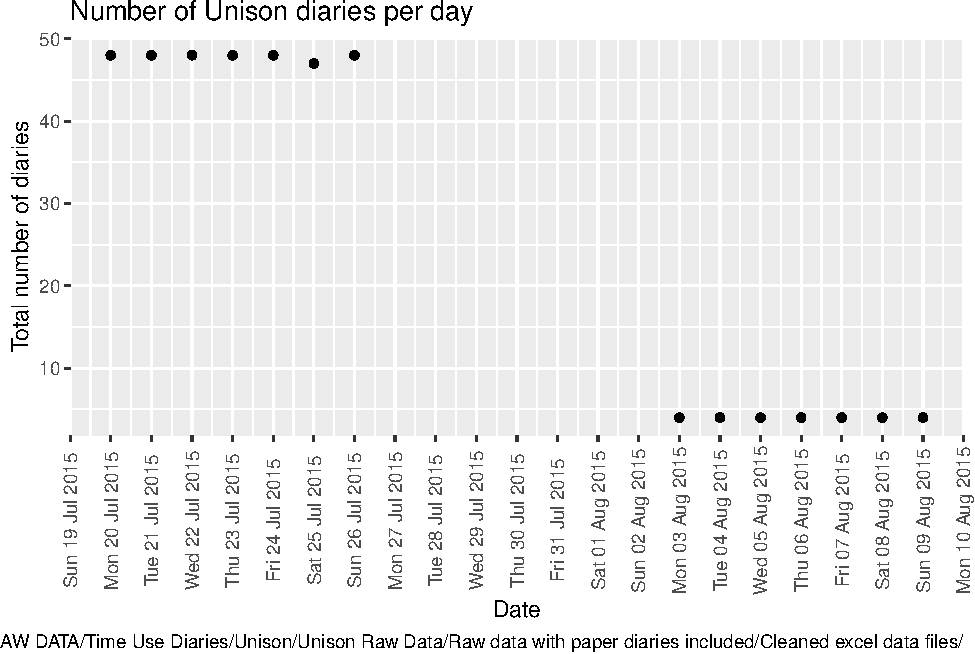
\includegraphics{processNZGGTUDData_files/figure-latex/unisonDiaryPLot-1.pdf}

\begin{verbatim}
## Saving 6.5 x 4.5 in image
\end{verbatim}

If any of them are earlier than July 2015 they are flagged below for
ease of fixing.

Table: Households with potential diary date errors

r\_diaryDate code tudCode sourceFile nDiaries ------------ -----
-------- ----------- ---------

\section{Summary}\label{summary}

Total responses:

\begin{itemize}
\tightlist
\item
  PowerCo - 352 diaries from 22 households for the period 2014-08-23 to
  2014-09-01.
\item
  Unison - 363 diaries from 20 households for the period 2015-07-20 to
  2015-08-09.
\end{itemize}

\section{Runtime}\label{runtime}

<<<<<<< HEAD
Analysis completed in 10.24 seconds ( 0.17 minutes) using
=======
Analysis completed in 16.42 seconds ( 0.27 minutes) using
>>>>>>> 8aad2b775c17c569a76cca0fc63e94e74b84bba0
\href{https://cran.r-project.org/package=knitr}{knitr} in
\href{http://www.rstudio.com}{RStudio} with R version 3.4.4 (2018-03-15)
running on x86\_64-apple-darwin15.6.0.

\section{R environment}\label{r-environment}

R packages used: data.table, lubridate, ggplot2, readr, dplyr, readxl,
knitr

\begin{itemize}
\tightlist
\item
  base R - for the basics (R Core Team 2016)
\item
  data.table - for fast (big) data handling (Dowle et al. 2015)
\item
  lubridate - date manipulation (Grolemund and Wickham 2011)
\item
  ggplot2 - for slick graphics (Wickham 2009)
\item
  readr - for csv reading/writing (Wickham, Hester, and Francois 2016)
\item
  dplyr - for select and contains (Wickham and Francois 2016)
\item
  knitr - to create this document (Xie 2016)
\item
  nzGREENGrid - for local NZ GREEN Grid utilities
\end{itemize}

\begin{verbatim}
## R version 3.4.4 (2018-03-15)
## Platform: x86_64-apple-darwin15.6.0 (64-bit)
## Running under: macOS High Sierra 10.13.4
## 
## Matrix products: default
## BLAS: /Library/Frameworks/R.framework/Versions/3.4/Resources/lib/libRblas.0.dylib
## LAPACK: /Library/Frameworks/R.framework/Versions/3.4/Resources/lib/libRlapack.dylib
## 
## locale:
## [1] en_GB.UTF-8/en_GB.UTF-8/en_GB.UTF-8/C/en_GB.UTF-8/en_GB.UTF-8
## 
## attached base packages:
## [1] stats     graphics  grDevices utils     datasets  methods   base     
## 
## other attached packages:
## [1] knitr_1.20          readxl_1.1.0        dplyr_0.7.4        
## [4] readr_1.1.1         ggplot2_2.2.1.9000  lubridate_1.7.4    
## [7] data.table_1.10.4-3 nzGREENGrid_0.1.0  
## 
## loaded via a namespace (and not attached):
##  [1] Rcpp_0.12.16      pillar_1.2.2      compiler_3.4.4   
##  [4] cellranger_1.1.0  plyr_1.8.4        highr_0.6        
##  [7] bindr_0.1.1       tools_3.4.4       digest_0.6.15    
## [10] evaluate_0.10.1   tibble_1.4.2      gtable_0.2.0     
## [13] pkgconfig_2.0.1   rlang_0.2.0.9001  yaml_2.1.18      
## [16] bindrcpp_0.2.2    withr_2.1.2       stringr_1.3.0    
## [19] hms_0.4.2         rprojroot_1.3-2   grid_3.4.4       
## [22] glue_1.2.0        R6_2.2.2          rmarkdown_1.9    
## [25] magrittr_1.5      backports_1.1.2   scales_0.5.0.9000
## [28] htmltools_0.3.6   assertthat_0.2.0  colorspace_1.3-2 
## [31] labeling_0.3      stringi_1.1.7     lazyeval_0.2.1   
## [34] munsell_0.4.3
\end{verbatim}

\section*{References}\label{references}
\addcontentsline{toc}{section}{References}

\hypertarget{refs}{}
\hypertarget{ref-data.table}{}
Dowle, M, A Srinivasan, T Short, S Lianoglou with contributions from R
Saporta, and E Antonyan. 2015. \emph{Data.table: Extension of
Data.frame}. \url{https://CRAN.R-project.org/package=data.table}.

\hypertarget{ref-lubridate}{}
Grolemund, Garrett, and Hadley Wickham. 2011. ``Dates and Times Made
Easy with lubridate.'' \emph{Journal of Statistical Software} 40 (3):
1--25. \url{http://www.jstatsoft.org/v40/i03/}.

\hypertarget{ref-baseR}{}
R Core Team. 2016. \emph{R: A Language and Environment for Statistical
Computing}. Vienna, Austria: R Foundation for Statistical Computing.
\url{https://www.R-project.org/}.

\hypertarget{ref-ggplot2}{}
Wickham, Hadley. 2009. \emph{Ggplot2: Elegant Graphics for Data
Analysis}. Springer-Verlag New York. \url{http://ggplot2.org}.

\hypertarget{ref-dplyr}{}
Wickham, Hadley, and Romain Francois. 2016. \emph{Dplyr: A Grammar of
Data Manipulation}. \url{https://CRAN.R-project.org/package=dplyr}.

\hypertarget{ref-readr}{}
Wickham, Hadley, Jim Hester, and Romain Francois. 2016. \emph{Readr:
Read Tabular Data}. \url{https://CRAN.R-project.org/package=readr}.

\hypertarget{ref-knitr}{}
Xie, Yihui. 2016. \emph{Knitr: A General-Purpose Package for Dynamic
Report Generation in R}. \url{https://CRAN.R-project.org/package=knitr}.


\end{document}
